\documentclass[10pt]{article}
\usepackage[utf8]{inputenc}
\usepackage[letterpaper,top=20mm,left=15mm,right=15mm,bottom=15mm]{geometry}
\usepackage{sectsty}
\sectionfont{\fontsize{10}{10}\selectfont}
\usepackage{graphicx} % Required for the inclusion of images
\usepackage[square,numbers]{natbib}
\bibliographystyle{apalike}
\setlength{\bibsep}{0.0pt}
\usepackage{times} % TNR font
\usepackage{multicol,caption}
\newenvironment{Figure}
  {\par\medskip\noindent\minipage{\linewidth}}
  {\endminipage\par\medskip}
\setlength{\columnsep}{0.6cm}
\usepackage{ragged2e} % allows \justify cmd

\begin{document}
\centering
\textbf{Abstract Template for ISB-ASB 2019} \par
\vspace{10pt}
\textbf{First I. Author$^1$}, Second I Author$^2$ \\
$^1$Faculty of Kinesiology, University of Calgary, Calgary, AB, Canada \\
$^2$Department of Mechanical Engineering, University of Calgary, Calgary, AB, Canada \\
Email: {anemail@ucalgary.ca} \vspace{5pt}

\begin{multicols}{2}
\justify
\textbf{Summary} \vspace{5pt} \newline
A brief summary (150 words maximum, plain text) should be included as the first section. The text of the summary should also be copy-pasted separately into the dedicated field within the online abstract submission system at the time of abstract submission. This summary will appear in the on-line program. \vspace{10pt} \newline
\textbf{Introduction} \vspace{5pt} \newline
This document serves as an abstract template and contains information about the abstract submission process. All abstracts must be submitted electronically via the official website of ISB 2019, by the deadline indicated. \vspace{5pt} \newline
The abstract should be prepared using the Microsoft Word or LaTeX template. All abstracts must be submitted as a PDF file and must not be larger than 5 MB. The congress organisers reserve the right to reject abstracts that do not adhere to this template. \vspace{10pt} \newline
\textbf{Methods} \vspace{5pt} \newline
The abstract is limited to one Letter size page (8.5$\times$11 in, 215.9$\times$279.4 mm), with two columns of text. The top margin should be 20 mm, while left, right and bottom margins should be 15 mm. The column width should be 90 mm. All text should be in font Times New Roman or Times, size 10 pt, except for the figure$/$table captions, which should be in size 9 pt. \vspace{5pt} \newline
The title (Sentence case bold), authors, and author affiliations should be centred across the top of the page. Use numerical superscripts to distinguish authors who are from different institutions. An email address of the corresponding author must be included. The \textbf{presenting author} should be in bold. \vspace{5pt} \newline
The text within each column should be right- and left-justified, without paragraph indentations. The body of the manuscript should be divided into sections such as Introduction, Methods, Results and Discussion, Conclusions (all words capitalized and bold). Spacing (already set in this template): 5 pt for the text, 10 pt before and 5 pt after for the section headers. \vspace{10pt} \newline
\textbf{Results and Discussion} \vspace{5pt} \newline
A maximum of two items, figures and/or tables, are recommended within the document. The figures or tables (if included) should be placed immediately after a paragraph and should be referenced parenthetically in the text (Figure 1). Captions should be placed below each figure and above each table. Tables may extend across two columns when needed, in which case they must be placed at the bottom of the page (Table 1). In Microsoft Word, use “Format $\rightarrow$ Columns” to control which parts of the text are in single column format.
\begin{Figure}
    \centering
    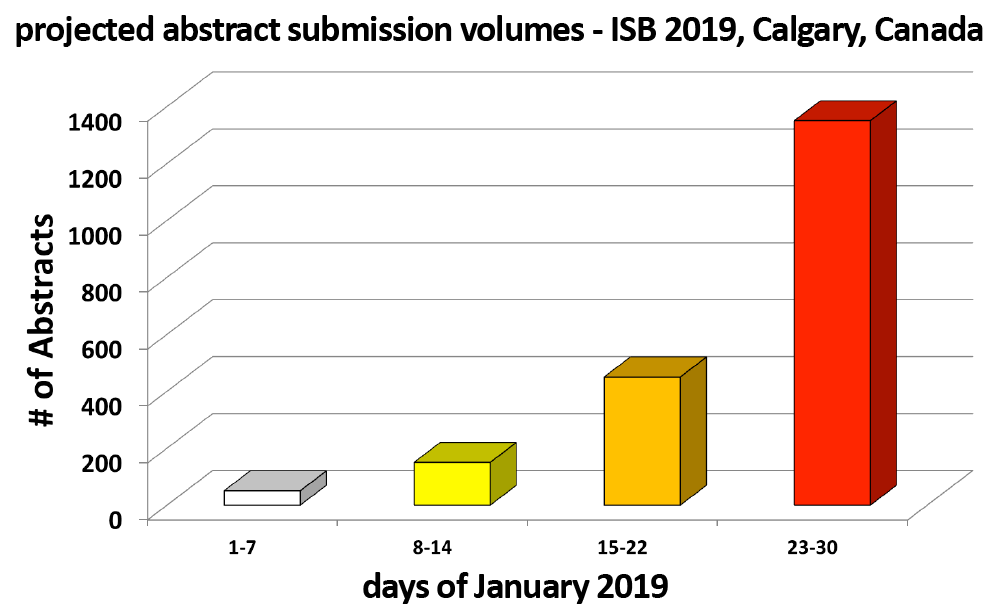
\includegraphics[width=\linewidth]{isb}
    \captionof{figure}{My caption}
\end{Figure}

\noindent
Reference citations within the text are to be made with numbers in square brackets \cite{Wilkinson2018a} \cite{Wilkinson2018b}. References are to be formatted as illustrated below. Place the journal or book title in Italics, with volume numbers in \textbf{bold} \cite{Wilkinson2018a}. \vspace{10pt} \newline
\noindent
\textbf{Conclusion} \vspace{5pt} \newline
In the event that an incomplete submission is received, it may be withheld from acceptance until the authors supply all required components. \vspace{10pt} \newline
\noindent
\textbf{Acknowledgments} \vspace{0.4em} \newline
Acknowledgments are optional and should specify research funding and resources including organization name and reference numbers (if applicable).
\bibliography{bibliography}
\end{multicols}

\begin{table}[h]
    \centering
    \caption{Interesting data from interesting experiments. The data have been arranged in an interesting manner.}
    \begin{tabular}{|c|c|c|c|c|}
    \hline
        Data & 234 & 23434 & 23 & 232323 \\
        \hline
        Other & 234 & 23434 & 23 & 232323 \\
    \hline
    \end{tabular}
    \label{tab:my_label}
\end{table}

\end{document}
